\documentclass[screen, compress]{beamer}
\usepackage[T1]{fontenc}
\usepackage[utf8]{inputenc}
\usepackage[english]{babel}
\usepackage{graphicx}
\usepackage{color} % text coloring
\usepackage{wrapfig} % Wrap text around figures
\usepackage{float} % position of figures
\usepackage{booktabs} % Professional tables
\usepackage{multirow} % Row spanning
\usetheme{Warsaw}

\title[TDT4215 project presentation]{TDT4215: Web-intelligence\\Group 1 project presentation}

\author[Group 1]{Group 1\\
Terje Snarby\\
Even Wiik Thomassen\\
Weilin Wang%
}

%Norges teknisk-naturvitenskapelige universitet
\institute[NTNU]{
\includegraphics[width=0.75\textwidth,height=0.22\textheight]{img/ntnu}}
%\institute[NTNU]{
\includegraphics[width=0.75\textwidth,height=0.22\textheight]{img/ntnu-no}}

\date{\today}

% 1. Explain the system architecture and function and role of the components.
% 2. Which components did you make yourself?
% 3. Present and discuss the results of algorithm.
% 4. Discuss (pros and cons) Explain the selected classification algorithm.
% 5. Evaluation of the classifiers.

\begin{document}

\begin{frame} % EVEN
\titlepage
\end{frame}


%=====================
\section{Introduction}
%=====================

%-------------------------------
\subsection{System architecture}
%-------------------------------
\begin{frame}{System architecture} % EVEN
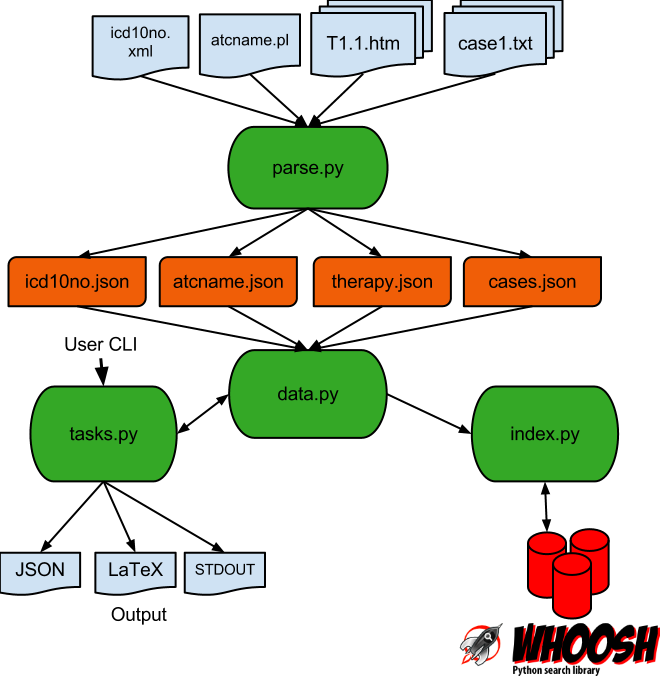
\includegraphics[width=\textwidth,height=0.92\textheight]{img/system_architecture2}
\end{frame}

%-------------------
\subsection{Workflow}
%-------------------
\begin{frame}{Workflow} % TERJE
	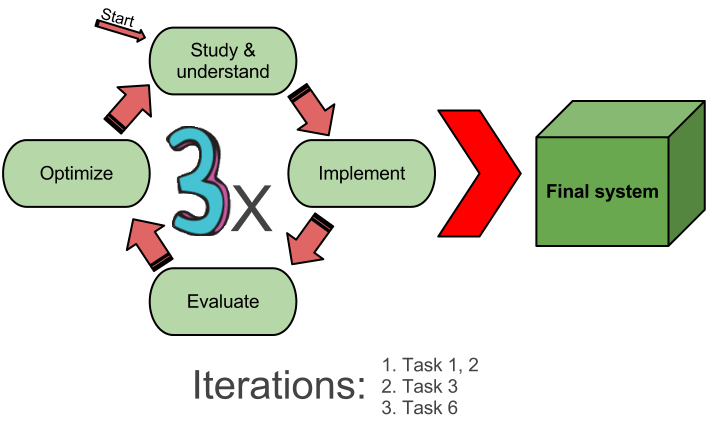
\includegraphics[width=\textwidth,height=0.9\textheight]{img/summary}
\end{frame}


%===============
\section{Method}
%===============

%--------------------------
\subsection{ICD-10 and ATC}
%--------------------------
\begin{frame}{Autocoding ICD-10 and ATC codes} % TERJE
\LARGE
\begin{itemize}
	\item Bag-of-words scoring algorithm
	\item BM25F
\end{itemize}
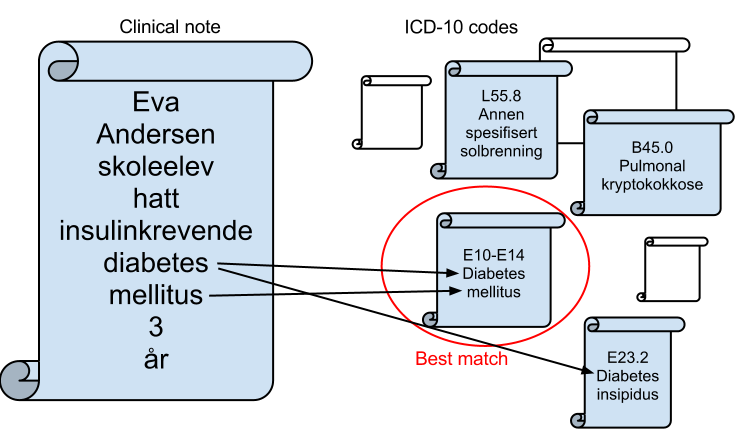
\includegraphics[width=\textwidth,height=0.7\textheight]{img/bagofwords}
\end{frame}

%------------------------
\subsection{Vector model}
%------------------------
\begin{frame}{Clinical notes and therapy chapter similarities} % TERJE
\Large
\begin{description}
	\item[Algorithm] Vector space model based on TF-IDF
	\item[Method A] log normalization and inverse frequency
	\item[Method B] log normalization and probabilistic inverse frequency
	\item[Method C] raw frequency and inverse frequency
	\item[Method D] raw frequency and probabilistic inverse frequency
\end{description}
\end{frame}

%---------------------------
\subsection{Improve results}
%---------------------------
\begin{frame}{How we improved the ranking} % Even
\Large
\begin{itemize}
	\item Aggregation and weighting of results
	\item Hierarchical nature of ICD-10 and ATC codes
	\item Hierarchical structure of therapy chapters
\end{itemize}
\end{frame}


%===============================
\section{Results and evaluation}
%===============================

%-----------------------------
\subsection{Result evaluation}
%-----------------------------
\begin{frame}{Improvement based on result evaluation} % EVEN
\begin{columns}
\begin{column}[l]{6cm}
{ \Large
\begin{itemize}
	\item Automatic evaluation of the whole system
	\item Feedback for optimizing classification algorithm
\end{itemize}
}
\end{column}

\begin{column}[r]{5cm}
\begin{table}
\begin{tabular}{c c c}
    \toprule
    Case & P@10 & R-precision \\
    \midrule
	1 & 70\% & 0.57 \\
	2 & 70\% & 0.86 \\
	3 & 100\% & 1.00 \\
	4 & 90\% & 0.89 \\
	5 & 90\% & 0.89 \\
	6 & 90\% & 0.89 \\
	7 & 90\% & 1.00 \\
	8 & 80\% & 0.88 \\
    \midrule
	Avg & 85\% & 0.87 \\
	\bottomrule
\end{tabular}
\end{table}
\end{column}
\end{columns}
\end{frame}

%-----------------------
\subsection{Our results}
%-----------------------
{
\usebackgroundtemplate{%
  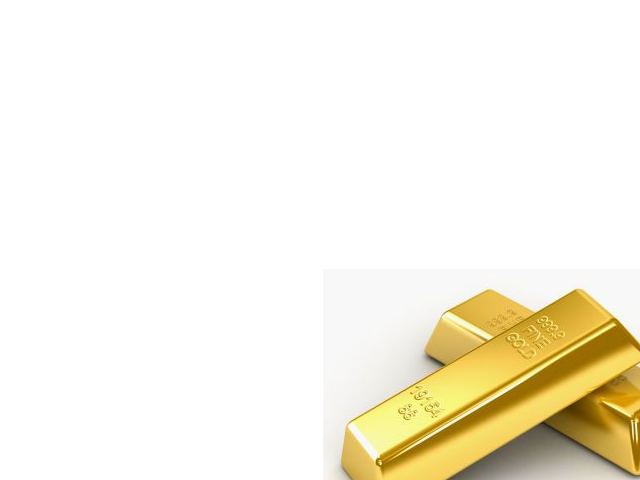
\includegraphics[width=\paperwidth]{img/gold}}
\begin{frame}{Our results versus gold standard} % WEILIN
\begin{table}
\begin{tabular}{c c l c}
    \toprule
    Case & Rank & Relevant chapter & Gold standard \\
    \midrule
    1 & 1 & {\color{blue}T3.1 Diabetes mellitus} & Yes \\
	\addlinespace
    2 & 1 & {\color{blue}T10.2 Obstruktiv lungesykdom} & Yes \\
     & 2 & T3.1 Diabetes mellitus & No \\
     & 3 & {\color{blue}T10.2.2 Kronisk obstruktiv} & Yes \\
	\addlinespace
    3 & 1 & {\color{blue}T1.10 Akutt bakteriell meningitt} & Yes \\
	\addlinespace
    4 & 1 & {\color{blue}T8.3 Koronarsykdom} & Yes \\
     & 2 & {\color{blue}T8.3.1 Stabil koronarsykdom} & Yes \\
     & 3 & T8 Hjerte- og karsykdommer & No \\
     & 4 & {\color{blue}T8.3.2 Ustabil koronarsykdom} & Yes \\
	\bottomrule
\end{tabular}
\end{table}
\end{frame}
}


%================
\section{Summary}
%================

%----------------------
\subsection{Discussion}
%----------------------
\begin{frame}{Discussion on our classification algorithm} % WEILIN
\begin{block}{Strengths}
\begin{itemize}
	\item Great results
	\item Multiple sources, more accurate results
	\item No training necessary
\end{itemize}
\end{block}

\begin{block}{Weaknesses}
\begin{itemize}
	\item Domain knowledge needed for optimal
	\item No feedback/learning.
	\item Consider asking a botanist: Is an object a tree?
\end{itemize}
\end{block}
\end{frame}

%-------------------
\subsection{Summary}
%-------------------
\begin{frame}{Summary} % Weilin
\begin{itemize}
	\item Implemented a working patient case search system
	\item Used vector based model
	\item Used automatic evaluation
	\item Almost perfect results in regards to gold standard
\end{itemize}
\end{frame}

%----------------------
\subsection{Questions?}
%----------------------
\begin{frame}{Questions?}
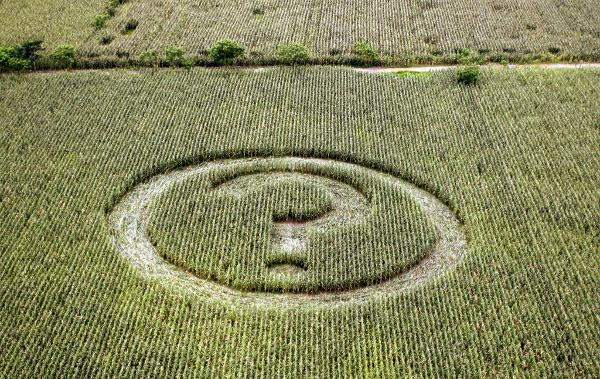
\includegraphics[width=\textwidth]{img/any-questions}
\end{frame}

\end{document}

